\documentclass[11pt,toc]{article}
\renewcommand{\familydefault}{\sfdefault}
\setcounter{secnumdepth}{6}
\usepackage[left=2cm,right=2cm]{geometry}
%\usepackage[document]{ragged2e} % Damit alles: Links aligned (der linkeste Punkt eines jeden Buchstaben ist auf einer Linie für alle zeilen) und so viel Platz nach rechts ausnutzt, wie möglich (nein, macht TeX nicht standardmäßig); muss man nicht für das gesamte Dokument machen (wie hier), geht auch per \raggedright oder \RaggedRight für/vor Paragraphen; gibt auch Umgebungen für rechtsbündigen Text https://de.overleaf.com/learn/latex/Text_alignment
\usepackage[dvipsnames]{xcolor}
\usepackage{booktabs,array}
\usepackage[author={Hendrik Theede}]{pdfcomment}
\usepackage{tabularx}
\usepackage{listings}
\definecolor{codegreen}{rgb}{0,0.6,0}
\definecolor{codegray}{rgb}{0.5,0.5,0.5}
\definecolor{codepurple}{rgb}{0.58,0,0.82}
\definecolor{backcolour}{rgb}{0.95,0.95,0.95}

\lstdefinestyle{mystyle}{
    backgroundcolor=\color{backcolour},   
    commentstyle=\color{codegreen},
    keywordstyle=\color{magenta},
    numberstyle=\tiny\color{codegray},
    stringstyle=\color{codepurple},
    basicstyle=\ttfamily\footnotesize,
    breakatwhitespace=false,         
    breaklines=true,                 
    captionpos=b,                    
    keepspaces=true,                 
    numbers=left,                    
    numbersep=5pt,                  
    showspaces=false,                
    showstringspaces=false,
    showtabs=false,            
    tabsize=2
}

\lstset{style=mystyle}



\usepackage{minted}
\usepackage{graphicx}
\usepackage{pdfpages} 
\usepackage{caption}
\usepackage{subcaption}




\usepackage[english,ngerman]{babel}
\usepackage[english=british]{csquotes}

\usepackage{tikz}
\usetikzlibrary{calc,positioning}
\usepackage{pgfplots}
\usepackage[nottoc]{tocbibind}
\usepackage{amsmath}

% Danke an https://tex.stackexchange.com/questions/14342/verbatim-environment-that-can-break-long-lines
\usepackage{fancyvrb}
\usepackage{fvextra}
% !!! Funktioniert nur mit ASCII-Zeichen (nicht mit deutschen Umlauten ä,ö,ü(,ß))

\usepackage{natbib}
\bibliographystyle{agsm}

%%% Uni-HRO relevantes
%%% TeX-relevant (siehe: titlepage.tex)
\author{Hendrik Theede}
\date{02.12.2025}
\title{Automatische Sprachübersetzung von \LaTeX{}-Dokumenten}
\def\matrikelnummer{221201256}
\newcommand{\supervisor}{Prof.\ Dr.\ rer.\ nat.\ habil. Clemens H. Cap}					% Betreuer
\newcommand{\ief}{Fakultät für Elektrotechnik und Informatik}							% Fakultaet
\definecolor{colorscheme}{cmyk}{0.90, 0.30, 0.00, 0.00} 								% Farbschema der Fakultaet; Siehe Corp. Design
\newcommand{\iuk}{Lehrstuhl für Informations- und Kommunikationsdienste}				% Institut



%%% "Deutsche Sprache"-relevant
\renewcommand*\contentsname{\hypertarget{toc}{Inhaltsverzeichnis}} % cannot contain \par (and thus: newlines)
\renewcommand*\refname{Literaturverzeichnis} % can contain \par (and thus: newlines)
\renewcommand*\figurename{Abbildung}



% Muss ans Ende, weil sonst übernimmt ein Biber aus der Bibliothek
\usepackage{hyperref}					% TeX!	
\hypersetup{
		linktoc=all,
		allcolors=black,
		colorlinks=true, % Für offizielle Releases das % vorne wegnehmen. Ersetzt die Boxen um Links durch die eigentlichen Farben
		linkcolor=black,
		urlbordercolor={1 0 0},
		urlcolor=blue, 
		citecolor=magenta,
		breaklinks=true,
		pdftitle=Abschlussarbeit,
		pdfauthor=Hendrik Theede,
		pdfsubject=Matrikelnummer 221201256,
		pageanchor,
		backref,
}

\begin{document}

\makeatletter % um \@author und co zu nutzen
\thispagestyle{empty}

\begin{figure}[h!]
\begin{tikzpicture}[remember picture,overlay,shift=(current page.south west)] 
	\begin{scope}
		% Koordinaten für Titel...
		\coordinate (A) at (3.7cm,20cm);
		% ... und Angaben
		\coordinate (B) at (3.7cm,3cm);
		
		% Uni-Logo
		\node [right] at (2cm,25cm) {
\includegraphics[width=12cm]{pictures/UNIHRO_LOGO_2025.pdf}};
		
		% Rahmen
		\draw[line width=2pt,colorscheme,rounded corners=2ex] (0cm,0cm) +(2cm,0cm) --(2cm,23.5cm) -- (19cm,23.5cm) -- (19cm,0cm);
		
		% Titel
		\node at (A) [below right] {\parbox{.85\textwidth}{\noindent\bfseries\sffamily{\Huge\raggedright \textcolor{colorscheme}{\@title}\par}}};
		
		% Angaben
		\node at (B) [above right] {\parbox{.85\textwidth}{
				\begin{tabular}{ll}
					Name: & \Large\@author				\\[2pt]
					Matrikelnummer: & \matrikelnummer					\\[1ex]
					Abgabedatum: & \@date				\\[5ex]
					Betreuer und Gutachter: & \supervisor  		\\[2pt]
					& Universität Rostock						\\[2pt]
					& \ief										\\
				\end{tabular}
			}
		};
		
		\fill[colorscheme] (0cm,0cm) +(2cm,0cm) rectangle (19cm,2cm);
		\path (3.7cm,1.5cm) [right,white] node{\Large\sffamily\textbf{\Large{Bachelorarbeit}} \small{am \iuk}};
		\path (3.7cm,.8cm) [right,white] node{\Large\sffamily\textbf{\ief}};
	\end{scope}
\end{tikzpicture}
\end{figure}
\makeatother



\pagenumbering{Roman}
\setcounter{page}{0}
\newpage
\newpage
\section*{Abstrakt}
placeholder
\newpage
\tableofcontents
\newpage
\pagenumbering{arabic}

\begingroup
\hypersetup{hidelinks,pdfborder={0 0 1},allbordercolors=magenta}% Hat länger gedauert, als mir lieb ist. sagt TeX: innerhalb dieser Gruppe sollen links nicht farbig sein. würde zuerst auch implizieren, dass keine Rahmen in der PDF angezeigt werden sollen. Wie löst man das? Indem man manuell sagt: Wir haben einen Rahmen um Hyperrefs mit Offset X = 0, Offset Y = 0 und Stärke in Pixeln: 1 (standard)

\section{Einleitung}
Wohingegen sich die Sprachübersetzung im Web schnell auf gängige Technologien wie DeepL oder Google's Gemini zurückführen lässt, zeigt sich eine ähnliche Übersetzung von \TeX{} und \LaTeX{} Dokumenten nur in ernüchternder Weise verfolgt. Lösungsansätze zu diesem Problem existieren bereits, allerdings gehen diese oftmals Umwege und trennen die Fähigkeiten der \TeX{}-Engine nicht in jedem Fall von den Technologien, welche verwendet werden sollen, um textliche Inhalte einer menschlichen Sprache in eine Andere zu übersetzen.\\
\noindent
Wo eine naive Nutzung solcher Software bereits im Alltag schnell Schwierigkeiten aufzeigt, ist insbesondere in einem wissenschaftlichen und mathematischem Kontext eine gezielte Verwendung der dieser Technologien erstrebenswert, sodass nicht jegliche Texte unabhängig voneinander und kontextlos übersetzt werden. Andernfalls wäre es denkbar, dass das deutsche Wort \enquote{ungerade} seine Bedeutung gegenüber einer mathematischen Operation verliert (nach welcher eine Zahl modulo 2 in 1 resultiert) und als umgangssprachliches \enquote{schief} interpretiert wird und im Englischen respektiv als \enquote{odd}, bzw.\ \enquote{crooked} übersetzt werden würde. Neben einer solchen Erhaltung von Kontexten ist auch eine selbstständige Erkennung der zu übersetzenden Sprache (Originalsprache eines Dokumentes) interessant, jedoch nicht zwingend erforderlich.\\
\noindent
Weiterhin dürfen Übersetzungsprozesse selbstverständlich nicht darin enden, dass eine entstehende (bspw.) PDF entweder vollständig unlesbar wird. % TeX Syntax kaputt
Daneben sollten allerdings auch keine unlesbaren Sektionen innerhalb der jeweiligen Dokumente entstehen, die aus von Layouting-Problemen resultieren, welche sich für die Übersetzung in einige Sprachen zeigen (jedoch in einigen Fällen unvermeidbar sind).\\ 
\noindent
Wünschenswert ist neben vorigen Aspekten auch Möglichkeiten für den Endnutzer zu erlauben, sollte dieser spezielle Übersetzungen oder Kontexte für einige Wörter wünschen, welche jedoch nicht aus dem Dokument selbst hervorgehen. % Schaffe ich es in dieser Arbeit das Wort "inhärent" NICHT zu verwenden?
Außerdem sollte ein möglichst hoher Support für sowohl verschiedene menschliche Sprachen, aber auch verschiedene \LaTeX{}-Pakete gegeben sein, wobei Letzteres nur ein Bonus ist, sollten Systeme wie Ti\textit{k}Z, bzw.\ \texttt{pgfplots} oder Bib\TeX{} innerhalb \LaTeX{} (zusammen mit \TeX{}) nutzbar bleiben.% Da sich durch diese sämtliche Verhalten anderer Pakete reproduzieren ließen.
%%%%% Kurzer Reminder für die wichtigsten Tücken (aber auch 'benefits' (EN für: Vorteil)) der deutschen Sprache für nativ dieser Sprache Mächtigen, welche nicht in wissenschaftliche Arbeiten fließen sollten. 
%%%%% 
%%%%% Meist recht offensichtlich.
%%%%%
%%%%% Konjunktiv 2: Impliziert meist eine Form von "Subjekt hätte etwas tun müssen" oder "Subjekt wird etwas tun" (oder schlimmer noch passiv: "mit Subject wird etwas geschehen", hier braucht es sogar das Partizip 2). Intuitiv wird klar, dass etwas nicht stattfand. Eine Quelle von möglicher Redundanz. Modalverben stehen oft in Verbindung mit solchen Implikationen ("dürfte ich etwas", "müsste ich etwas", "könnte ich etwas"... meist: ja, theoretisch gesehen "kann" man alles. Daher nicht schreiben: "man müsste/könnte/sollte etwas [so und so] machen", sondern: "A existiert, wodurch sich B ergibt). Siehe: Konditionalsätze
%%%%% Konzessivsätze: Leicht am Konjunktiv 2 zu erkennen. "Entgegen Behauptung X, ist die Realität Y". Die Realität gehört an den Anfang und aus dieser sollte genug Information hervorgehen, dass Behauptung X nicht ausformuliert werden muss.
%%%%% 
%%%%% Implikationen: Erklärung bedürfte eigentlich einem (mir noch unbekanntem) wissenschaftlichen Teilgebiet der "Aussagentheorie". Entspringt der Modularität deutscher Substantive ("Rindfleischetikettierungsüberwachungsaufgabenübertragungsgesetz" als Beispiel. Wir beschäftigen uns mit der Rindfleischetikettierung, welche überwacht werden soll. Das "s" nach "Rindfleischetikettierung" entstammt einem implizierten Genitiv (Überwachung der Rindfleischetikettierung = Rindfleischetikettierungsüberwachung), genauso wie das "s" nach "[...]überwachung[...]" (Aufgabenübertragung (bei) der Überwachung). Letztendliches "s" vor "[...]gesetz" ist am einfachsten, da sich Gesetze immer auf etwas beziehen. "Ein Gesetz einer Sache" kann zu "Gesetz der Sache" vereinfacht werden, aus welcher der Genitiv wieder hervorgeht).  

%%%%% Konditionalsätze: 
%%%%% "Aus These X, folgt Hypothese". "Daher folgt die nächste Hypothese". (Hypothese = These, welche auf einer anderen These aufbaut. Grundlage der Mathematik)
%%%%% Formal entweder eine Bedingung in einem Nebensatz (if-else statement) oder Schlussfolgerung in einem Hauptsatz (Folgesatz, vergleichbar: Zuweisungen). 
%%%%% - Arten: Real und Irreal = Erfüllbare und nicht erfüllbare Bedingungen. 
%%%%% - meint: Solange ich atme, bin ich. (Wenn ich für immer aufhören würde zu atmen, wäre erste Bedingung nicht mehr erfüllt. Ich bin ein Mensch, daher stimmt die Aussage.)
%%%%% - meint: Gäbe es keine Luft, wäre ich nicht. (Annahme: Die Luft bleibt uns vorerst noch einatembar erhalten)
%%%%% - meint: Hätte es nie Luft gegeben, hätte es mich nie geben können. (Wir schließen den Kreis zu Konjunktiv 2 und bemerken das Plusquamperfekt).

%%%%% Plusquamperfekt: Als ich (etwas) tat, war (etwas anderes) bereits passiert. Oder Konditionalsatz mit Konjunktiv 2: Wäre (etwas) nie geschehen, hätte (Resultat) nie erscheinen können. Passiert umgangssprachlich oft "hätte ich (das und das [besser]) gemacht, hätte ich (das und das) bereits erreicht" bspw.: "Hätte ich keinen zweiten Versuch für eine Abschlussarbeit benötigt, hätte ich bereits den Studiengang beenden können. (Hier bemerkt man direkt: "beenden können" kann zu "beendet" gekürzt werden. Partizip II ist meist umgangssprachlich, da textlich nicht von Nöten).


%%%%%%%%%%%%% Versuche die deutsche wissenschaftliche Sprache verständlich zu halten:
%%%%%%%%%%%%% - Infinitiv so oft wie möglich (durch Substantivierung oder Erweiterung).
%%%%%%%%%%%%% - Reale Konditionalsätze nutzen

% Welche Arten von Fehlern können entstehen? (Was fällt einem auf, wenn man Dokumente schreibt und sich denkt: mmmmhh würde google translate das richtig übersetzen)
\section{Problemfälle}
Eine einzige, feste \TeX{}-Syntax existiert theoretisch gesehen nicht, wie ein~\hyperref[problems:advanced:catcode]{späterer Paragraph} aufzeigen wird.% So gehen in-document refs ganz gut.
Die Fähigkeit jegliche erdenkliche Zeichenkette (gegeben:\ diese ist auf einem Rechner darstellbar, siehe:~\cite{unicode}) sorgt zunächst für eine unendliche Menge an testbaren Problemen. Da es unmöglich ist eine unendliche Menge an Testfällen abzudecken, wird zunächst nur die vorgesehene \LaTeX{} (bzw.\ \TeX{}~Syntax nach~\cite{texbook}) betrachtet und die bereits rein innerhalb dieser schnellig auffallenden Fehler aufgezeigt, welche durch fälschlich übersetzte Zeichenketten entstehen könnten.\\\noindent
% reviewed: 1
% 
\subsection{Struktur}\phantomsection\label{problems:structure}% Warum Kategoriesieren?
\subsubsection{Klassifizierung}
Für spätere Testzwecke wurden die verschiedenen Problemfälle in einzelne Kategorien getrennt. Eine solche Kategorisierung ist technisch gesehen nicht zwingend, soll allerdings zur Verbesserung einer späteren Übersicht dienen. Die Einteilung konzentriert sich vorrangig auf die Komplexität des Problemes und in einer Reihenfolge, in welcher sie auch bei der Nutzung von \TeX{} für ein beliebiges Dokument auftreten könnten. 
%
% Definition: Direkte Probleme
Hierbei seien \textit{direkte Probleme} zunächst eher simple und technisch leicht zu behebende Probleme, welche sich durch ein einheitliches Vorgehen beheben lassen könnten.% Könnten muss an dieser Stelle so folgen
Zudem beschränkt man sich hier nur auf den benötigten Zugriff auf eine einzelne Datei.
%
% Definition: Indirekte Probleme und Zusammenfassung zu "simplen Problemen"
\textit{Indirekte Probleme} formen potentielle Schwierigkeiten, da sie einen Zugriff auf weitere Dateien benötigen, da sie von einer Ausgangsdatei referenziert werden. Technisch gesehen sind sie jedoch auch durch einheitliche Paradigma zu bewältigen. Daher werden sie im Kapitel~\ref{problems:simple} zusammengefasst und fortan als \enquote{simple Probleme} bezeichnet.
%
% Definition: Fortgeschrittene Probleme
\enquote{Fortgeschrittene Probleme} beziehen sich auf Probleme, welche sich paradigmatisch lösen lassen, % man kann einen Quellcode schreiben; paradigmatisch = Mustern folgend
aber zusätzliches Vorwissen verlangen. Dieses Vorwissen lässt sich bei diesen Problemfällen jedoch ermitteln, da der Entstehungsweg dieses Wissens nachvollziehbar ist.% Meint: Wir gucken uns an, wo und wann zu übersetzende Wörter hinter Makros, in Paketen, anderen >>Programmen<< versteckt wird.
\enquote{Speziellere Probleme} umfassen Probleme, welche sich nicht ohne Vorkenntnis des tatsächlichen Dokumentes beheben lassen. Nach diesen wird zudem noch auf ein paar rein sprachliche Schwierigkeiten eingegangen, welche unter Anderem zu solchen speziellen Problemen führen könnten.

\subsubsection{Beschreibung}
Jeder Problemfall wird zunächst durch ein Beispiel demonstriert\footnote{welche aus einem Test mit Hilfe von Google Translate in Firefox durchgeführt wurden (Oktober 2025)}, danach wörtlich in einer Beschreibung erläutert und wird abschließend abstrahiert und versucht auf konkrete \TeX{} Primitiven zurückgeführt zu werden. Die fortgeschritteneren Probleme bedürfen teilweise mehreren Beispielen zur Beschreibung, lassen sich jedoch auf ähnliche Äußerungen zurückführen. Einführende Beispiele werden in der Form \texttt{ausführbarer Code} wird zu \texttt{ausführbarer Code} übersetzt, aber \texttt{ausführbarer Code} zu \texttt{fehlerhafter Code}\footnote{\enquote{Code} bezieht sich in beiden Fällen auf \TeX{}-Quelltexte} (1-dimensional). Einige Beispiele benötigen mitunter eine 2-dimensionale Darstellung, da sie mehrere Zeilen Quellcode umfassen und werden tabellarisch nebeneinander gestellt~\pdfcomment[color=red, icon=Paragraph]{Evtl.\ werden alle Beispiele in tabellarische Form überführt, welche ich persönlich anschaulicher finde, jedoch mehr Platz rauben würde}. Einige Probleme auf höherer Abstraktionsebene lassen sich allerdings nur schwierig veranschaulichen, wodurch Beispiele sich teils wieder auf Schilderungen von Situationen berufen, um diese Übersicht übersichtlich zu halten.% valider Grund

% Namensgebung aus ~/tests/readme.md wahrscheinlich geeigneter
\subsection{Translative}\phantomsection\label{problems:simple}
% 0d zu 1d
\subsubsection{Unbekannte Wörter}\phantomsection\label{problems:dim0}
\verb|\label{problem:encounter:solve}| wird zu \verb|\label{Problem:Begegnung:Lösung}| übersetzt,\\aber \verb|\section{example}| zu \verb|\Abschnitt{Beispiel}|.
\paragraph*{Beschreibung}
\paragraph*{Abstrahierung}
Teile der \TeX{}-Syntax lassen sich anhand von \verb|\|, \verb|{|, \verb|}|, \verb|[|, \verb|]|, \verb|$|, \verb|$$| oder \verb|\%| erkennen und müssten daher ausgeschlossen werden. Man kann sich diese Art von Fehlern wie 0-dimensionale Fehler vorstellen, wobei die nullte Dimension hierbei bei einem einzelnen Wort beginnt (welche als Punkte zu verstehen sind).

% 0d zur ersten Dimension
\subsubsection{Auszulassende Wörter}\phantomsection\label{problems:dim1}% Meint: Wort wurde nicht als Syntaktisch relevant erkannt
\verb|\begin{myenvironment}[fontsize=red]| wird zu \verb|\begin{myenvironment}[fontsize=red]| übersetzt,\\aber \verb|\begin{myenvironment}[ fontsize = red ]| zu \verb|\begin{myenvironment}[ fontsize = rot ]|.
\paragraph*{Beschreibung}
\paragraph*{Abstrahierung}
Teile der \TeX-Syntax lassen sich nicht nur anhand der~\hyperref[problems:unexpectedCharacters]{zuvor} beschriebenen Zeichenketten erkennen, sondern lassen sich auch in Zeilen wiederfinden. Diese Art von Fehlern bahnt den Weg zu einer Dimension, wodurch nicht nur innerhalb eines Wortes (Punktes), sondern auch zwischen verschiedenen Punkten Fehler entstehen könnten (also innerhalb einer Zeile).

\newpage

% Vertikales Spacing / Zweite Dimension
\subsubsection{Neuartige Satzarten}\phantomsection\label{problems:dim2}
\begin{table}[h!]
    \centering
    \begin{tabularx}{\textwidth}{X X}
        \toprule
            Original & Übersetzung\\
        \midrule
        % Siehe ~/tests/readme.md für namensgebung und "Wo ist die Datei?"
            Beispiel 1\lstinputlisting[language=tex]{../examples/simple/2d/correct_original.tex} & \lstinputlisting[language=tex]{../examples/simple/2d/correct.tex}\\[2em]
            Beispiel 2\lstinputlisting[language=tex]{../examples/simple/2d/wrong_original.tex} & \lstinputlisting[language=tex]{../examples/simple/2d/wrong.tex}\\
        \bottomrule
    \end{tabularx}
    \caption{Beispiel für eine Zeile, welche übersetzt werden darf}\phantomsection\label{tab:problems:dim2}
\end{table}


\paragraph*{Beschreibung}
% Zwar ist es praktisch, wenn Quelltexte durch zusätzlichen Whitespace nicht nur auf horizontaler, sondern auch auf vertikaler Ebene übersichtlicher werden, allerdings führt dies bei einer zeilenweisen Übersetzung dazu, dass der Kontext aus voriger Zeile evtl. verloren geht.
\paragraph*{Abstrahierung}
Teile der \TeX-Syntax lassen sich nicht nur anhand von einzelnen Zeilen oder Zeichenketten erkennen, sondern könnten sich auch auch in verschiedenen Zeilen wiederfinden lassen. Diese Art von Fehlern kann 2-dimensional betrachtet werden, wodurch Fehler auch zwischen Zeilen entstehen können.

\newpage

% Dreidimensionales Spacing
\subsubsection{Größere Sprachstrukturen}\phantomsection\label{problems:dim3}
\paragraph*{Beispiel}
\begin{table}[h!]
    \centering
    \begin{tabularx}{\textwidth}{X X}
        \toprule
            Original & Übersetzung\\
        \midrule
        % Siehe ~/tests/readme.md für namensgebung und "Wo ist die Datei?"; hoffentlich sieht sich der Herr Prof. Dr. rer. nat. habil. nicht den Quellcode an dieser Stelle an.
            Datei $x$ & \\ 
            \lstinputlisting[language=TeX]{../examples/simple/3d/x_original.tex} & \lstinputlisting[language=tex]{../examples/simple/3d/x.tex}\\[2em]
            Datei $y$ & \\ 
            \lstinputlisting[language=TeX]{../examples/simple/3d/y_original.tex} & \lstinputlisting[language=tex]{../examples/simple/3d/y_original.tex}\\% Begründung, warum hier zwei mal nur ein und dieselbe Datei verwendet wird, ist dieser Datei zu entnehmen
            % edited "y_original.tex" ~12 h later: "has" has been replaced with "have". mistake was made, because i was thinking of one (or any) text, but forgot that i was referring to two versions syntactically. 
        \bottomrule
    \end{tabularx}
    \caption{Beispiel für eine übersehene Datei}\phantomsection\label{tab:problems:dim3}
\end{table}
\paragraph*{Beschreibung}
Die Übersetzung von Datei $x$, welche Datei $y$ via \texttt{input} oder \texttt{include} % Unterschied: input darf vernested werden, include nicht. wir gehen von einem größeren Werk aus, welches aus x Kapiteln besteht, welche integriert werden sollen. die einzelnen Kapitel werden danach nur in Abschnitte zerlegt, welche durch inputs eingebunden werden sollen
führt zwar dazu, dass Datei $x$ übersetzt wird, aber Datei $y$ nicht.
\paragraph*{Abstrahierung}% Hier war abstrahieren leichter als beschreiben
Teile der \TeX-Syntax müssen nicht zwingend in einer Datei vorliegen, sondern könnten auch in verschiedenen Dateien integriert sein. Die Klassifizierung simpler Probleme gelangt in \TeX{} hier bereits in der dritten Dimension an, weswegen sich fortan bereits mit \enquote{fortgeschrittenen} Problemen beschäftigt werden muss (welche sich Teils über mehrere \enquote{Dimensionen} erstrecken). Eine vierte Dimension existiert physikalisch nicht, ist jedoch mathematisch formulierbar\footnote{physikalisch: die vierte Dimension ist die Zeit, wenn man eine nicht-euklidische 3-dimensionale Bewegung verlangt (Teleportation)} und äußert sich in diesem Kontext auf eine Erhöhung von Laufzeitkomplexitäten.

\subsection{Technische Probleme}\phantomsection\label{problems:advanced}
%%% Hier ein wenig weg von der eigentlichen Struktur, jedoch für die konkreten Beispiele wieder gleich
\subsubsection{Hilfsdateien}% multi-file handling
\paragraph{Struktur dieses Abschnittes}
Eine Datei nutzt ein Literaturverzeichnis (Bib\TeX{}), pdf\TeX{} (\verb|\pdfcomment{}|), \verb|\footnote|, ein Inhaltsverzeichnis, ein Glossar, 

\paragraph{Beispielliste}
\subparagraph*{Inhaltsverzeichnisse, Abbildungsverzeichnisse, Tabellenlisten}
\paragraph*{Beispiel}
\paragraph*{Erläuterung}
Ändern wir den Titel eines Paragraphen oder Abschnittes, dann erfasst dies der \TeX{} Compiler beim ersten Durchlauf. Jedoch der String im Inhaltsverzeichnis kann nur verändert werden, sobald diese Information zu Beginn des nächsten Kompilierungsprozesses in der entsprechenden Hilfsdatei vorliegt (\texttt{.toc}).

\subparagraph{Backrefs}
\paragraph*{Beispiel}
Bedarf evtl.\ einer bildlichen Veranschaulichung. Meint: Inhaltsverzeichnis, Tabelle,\ldots vor einer \textit{backwards reference} verschiebt die echte Position der (Phantom-) Sektion. Daher muss zunächst bestimmt werden, wo im Dokument eine Referenz auf ein existierendes Label stattfindet, welches vorherig bereits vergeben wurde\pdfcomment{Ein Erneuern eines Labels via renewcommand ergibt keinen Sinn, da dieses forward references verfälschen würde.}.
\paragraph*{Erläuterung}
Ein Verweis auf einen vorherigen Paragraphen kann nur klickbar verlinkt werden, wenn die Information, an welcher Stelle er sich im Dokument befindet, bereits klar ist. Da nach der Referenz weitere Abschnitte folgen können, welche vorherige Elemente mit variabler Größe verändern könnten, muss zunächst die Größe dieser bestimmt sein und gegenüber dieser kann dann der 

\subparagraph*{Literaturverzeichnisse}
\paragraph*{Beispiel}
\paragraph*{Erläuterung}

\subparagraph*{PDF Funktionen}
\paragraph*{Beispiel}
\paragraph*{Erläuterung}

\subparagraph*{\enquote{footnotes}}
\paragraph*{Beispiel}
\paragraph*{Erläuterung}






\paragraph{Abstrahiertes Problem}
Falls auf Hilfsdateien zugegriffen wird, ist das mehrfache Kompilieren eines \LaTeX{} Dokumentes unvermeidbar. Gegeben $n_{h}$ womoglich existierenden Hilfsdateien, welche alle ihrerseits zu übersetzende Inhalte beinhalten können, folgt eine minimale Laufzeit $\mathcal{O}(n_h)$. 
%Ein einmaliges Kompilieren eines \LaTeX{} Dokumentes ist unmöglich, falls ein Zugriff auf Hilfsdateien nötig ist.


%%%%%%%%%% Für später relevant, für Makros und beliebige Nutzereingaben etc......:!:!:!!::!!::!
%Die Möglichkeiten andere Dateien in einem \LaTeX{} Dokument einzubeziehen, könnten nähern sich einer Unendlichkeit.% Warum? ist schwer zu beantworten, daher sollte man sich zunächst vor Augen führen, für welche Zwecke man auf andere Dokumente innerhalb eines Dokumentes verweisen möchte. // Warum eine Unendlichkeit? Es gibt unendlich viele Unendlichkeiten. Beweis bitte von Prof. Cap
%Ein Beschäftigen mit dieser führt zu nichts\footnote{invers},%, sodass zunächst die Frage gestellt werden müsste, wie diese entstehen können, indem alle denkbaren Arten, wie sich zwei oder mehrere Dateien gegenseitig referenzieren/benötigen könnten, aufgelistet wird. 
%weshalb ein Betrachten möglicher versteckter interner Abhängigkeiten zwischen verschiedenen \LaTeX{} Dokumenten unabdingbar ist.% [...], hence describing the possible internal dependencies of \LaTeX{} documents is necessary. // um von der Formulierung "weshalb mögliche interne Abhängigkeiten zwischen verschiedenen Dateien erläutert werden müssen" wegzukommen, sah ich mich gezwungen in die englische Sprache auszuweichen (da es mir dabei half zu erkennen, wie ich einen direkten Konjunktiv II vermeiden kann).
%%% Inwiefern wirkt sich das auf die gegebene Problematik aus
%Nur einen Teil eines Dokumentes zu übersehen, provoziert kontextuellen Verlust für Übersetzungen (Abschnitt~\ref{problems:dim3}). 
%\begin{enumerate}
%%    \item Permutationen (insgesamt 4, da wir nur zwischen $1$ und $n \textit{(beliebig vielen)}$ zu wechseln wünschen (2*2 Optionen / Urnen=1;Kugeln=2;Farben=2;zurücklegen)): 
%    \item Ein Dokument kann ein Anderes in sich tragen. 
%    \item Ein Dokument kann n Andere in sich tragen
%    \item n Dokumente können ein Anderes in sich tragen
%    \item n Dokumente können n Andere in sich tragen geht aus den beiden vorigen statements hervor und ist redundant (weil wir kennen bereits 1 dokument, welches n Andere tragen kann).
%\end{enumerate}
% Realität es gibt nicht unendlich viele Dokumente, da physikalisch nicht möglich (Archimedis). 
%Hier stoßen wir 


%%% Meint: Hier müssen wir die eigentlichen Literaturverweise kennen, um einen Kontext zu kennen.
\subsubsection{Unerreichbare Informationen}

\paragraph*{Beispiele}
\begin{table}[h!]
    \centering
    \begin{tabularx}{\textwidth}{X X}
        \toprule
            Original & Übersetzung\\
        \midrule
        % Siehe ~/tests/readme.md für namensgebung und "Wo ist die Datei?"; hoffentlich sieht sich der Herr Prof. Dr. rer. nat. habil. nicht den Quellcode an dieser Stelle an.
            Dokument & \\
            \lstinputlisting[language=TeX]{../examples/advanced/literature/example_original.tex} & \lstinputlisting[language=tex]{../examples/advanced/literature/example.tex}\\[2em]
            Bibliothek & \\
            \lstinputlisting[language=tex]{../examples/advanced/literature/example_original.bib} & \lstinputlisting[language=tex]{../examples/advanced/literature/example.bib}\\
            %%% Bemerkung: Übersetzung noch nicht erstellt.
        \bottomrule
    \end{tabularx}
    \caption{Beispiel für einen verpassten literarischen Kontext}\label{tab:problems:nonexisting}% mit reference 
\end{table}

\paragraph*{Beschreibungen}
Ein Dokument erwähnt ein Werk, in welchem es um die C-Programmierung geht. Rein aus den im System vorliegenden Dateien ist kein Kontext für das Wort \enquote{String} erkennbar, sodass ein Zugriff auf eine externe Ressource unabdingbar ist.

% Bemerkung: Nur die Suche (google.com) nach "salomon c programmierung" führt bspw. Gemini zu einer vermuteten Verwechslung mit dem Begriff "System" (Stand: 09.10.2025, 12:29).
% ISBN führt zur gleichen Minute direkt zum Institut (Angewandte Mikroelektronik und Datentechnik)... wobei Thalia denkt, dass ich "1984" online kaufen möchte...
\paragraph*{Abstrahierung}
Einfache Cloud-Architektur. Ein Client möchte auf ein beliebiges Wissen einer Webseite (bzw.\ dem Server und den beanspruchten Speicherplätzen in einem (beliebigen) Rechenzentrum\footnote{Hierbei ist nicht von Festspeicher zu reden. Aus Sicherheitsgründen sei davon auszugehen, dass sich die physischen Adressen des wissensrepräsentierenden Speichers regelmäßig und unvorhersehbar ändern} zugreifen).




\subsubsection{Figuren und Tabellen}\phantomsection\label{problems:advanced:tables}
\paragraph*{Beispiele}
\paragraph*{Beschreibungen}
\paragraph*{Abstrahierung}

\subsubsection{Literaturverzeichnisse}\phantomsection\label{problems:advanced:bibtex}
\paragraph*{Beispiele}
\paragraph*{Beschreibungen}
Bib\TeX{} erlaubt es an vielerlei Stelle eigene Strings in einer kompilierten \TeX{}-Datei zu verbergen.
\paragraph*{Abstrahierung}


\subsubsection{Category Codes}\phantomsection\label{problems:advanced:catcode}
\paragraph*{Beispiele}
\paragraph*{Beschreibungen}
\paragraph*{Abstrahierung}


\subsection{Spezifischer Technologien}\phantomsection\label{problems:special}
Mitunter NP-schwer.
\subsubsection{Kommentare}\phantomsection\label{problems:advanced:comments}
\paragraph*{Beispiele}
\paragraph*{Beschreibungen}
%- zunächst als Unterklasse von~\ref{problems:unexpectedCharacters} zu erwarten
%- kann jedoch auch~\ref{problems:verticalSpacing} umfassen
Wohingegen sich~\ref{problems:advanced:comments} nicht mit anderen, in Kommentaren referenzierten, Dateien beschäftigt, soll sich hier auf solche Fälle konzentriert werde.
\paragraph*{Abstrahierung}
Hier treffen simple Fehler aus den ersten drei Kategorien (in~\ref{problems:dim0},~\ref{problems:dim1} und~\ref{problems:dim2} geschildert) aufeinander. In die dritte Dimension, also in andere Dateien, wird jedoch (\hyperref[problems:special:comments]{vorerst}) nicht traversiert, da auskommentierte Datei-Einbindungen nicht erfasst werden dürften. 
Ausgehend von~\ref{problems:advanced:comment} wird nun erwartet, dass eine Referenzierung von Dateien erwartet wird, welche sich in Kommentaren verbergen. Dies kann jedoch~\ref{problems:special:sourcecode} beinhalten.


\subsubsection{Dilemmatische Makros}\phantomsection\label{problems:special:macrodilemma}
\paragraph*{Beispiele}
\paragraph*{Beschreibungen}
\paragraph*{Abstrahierung}

\subsubsection{TikZ und Layouting}\phantomsection\label{problems:advanced:layouting}
\paragraph*{Beispiele}
\paragraph*{Beschreibungen}
\paragraph*{Abstrahierung}

\subsubsection{Quellmehrsprachigkeit}\phantomsection\label{problems:special:sourcecode}
\paragraph*{Beispiele}
\paragraph*{Beschreibungen}
\paragraph*{Abstrahierung}
Quelltexte anderer Quellsprachen (Programmiersprachen) können ihrerseits auf andere Dateien verweisen, oder andere Syntaktik tragen. Das Erkennen dieser ist theoretisch gesehen leicht, jedoch praktisch gesehen schnellig zu übersehen. 









\subsection{Sprachliche Schwierigkeiten}\phantomsection\label{problems:additional}
\subsubsection{Glossare und Nomenklaturen}
\paragraph*{Beispiele}
\paragraph*{Beschreibungen}
\paragraph*{Abstrahierung}

\subsubsection{Weitere}
\paragraph*{Beispiele}
\paragraph*{Beschreibungen}
\paragraph*{Abstrahierung}

%\section{Technologischer Stand}
\subsection{Generische, fundamentale Technologien}
Den vorigen Abschnitt beginnend wurde Google Translate zur Erläuterung herangezogen, da sich mit dieser Ressource recht einfach typische Fehler aufzeigen, welche dem zugrundeliegen, dass Software dieser Art, bzw.\ in der Art, wie sie verwendet wurde, nicht davon ausgeht Strings einzulesen, welche kein Teil einer menschlichen Sprache sind, wie zum Beispiel \verb|{Beispiel}|. Ein Mensch kann hierbei die Klammern ignorieren, ein Computer oder ein Programm ohne Weiteres jedoch nicht.% Passt im Kontext Programm recht gut in dieser Formulierung. 
Jedoch basieren heutige Technologien zur Sprachübersetzung nicht mehr auf Programmen, welche einen festen Input mit syntaktischen Vorgaben erwarten, sondern auf weitaus mächtigerer Software, welche je nach erforderlichem Use-Case eine andere Art an Input erwartet. Als Endnutzer würde man sich zunächst jegliche Optionen offen halten wollen, wodurch man recht schnell bei den Technologien größerer und bekannter Anbieter angelangt, welche Anwendungs- und Nutzerschnittstellen für ihre Sprachmodelle anbieten. Von den Dingen, welche aus marktwissenschaftlicher Argumentation heraus direkt weniger vielversprechend sein \textit{müssten} (da diese Anbieter andere Software zur Dokumentenerstellung produzieren, welche sie verständlicherweise gegenüber einen kostenfreien Technologie wie \TeX{} in den Vordergrund stellen möchten), wird zunächst noch nicht abgesehen, sondern jegliche denkbare Technologie hinsichtlich ihrer potentiellen Möglichkeiten betrachtet. 

\paragraph*{ChatGPT}\label{par:chatgpt}
Der von OpenAI präsentierte statistische Ansatz zur Entwicklung einer künstlichen Intelligenz ist ein im ersten Moment naheliegender Ansatz, da man sich hier erhoffen könnte, dass diese Technologie mit Hilfe eines passenden \enquote{Prompting} auf längere Zeit gesehen sowohl qualitativ hochwertige Übersetzungen erzielt, als auch geschickt jede \TeX{}-Syntax geschuldete Hürde umgeht. Allerdings scheitert dieser Ansatz% zum Glück
bereits konzeptionell, denn der \TeX{}-Compiler (jeder) selbst wird dazu in der Lage bleiben \textit{nur} reine Zeichenketten von Befehlen, Makros und Ähnlichem zu unterscheiden, da diese ansonsten nicht wie gewünscht in einem Dokument als solche Zeichenkette vorzufinden wären. Da dieses Programm selbst auch deterministisch arbeitet (und arbeiten muss), benötigt man an dieser Stelle noch keine Einbindung einer potentiellen Fehleranfälligkeit.



% Hier beginnen die genauen! Fehler zu zeigen, jeweils an den Softwares

%%% Kurze Bemerkung zur Fragestellung jeweils:
%%% Wie sieht die API aus? Kann man überhaupt Kontext (z.B. TeX, in TeX geschrieben, ...) mitgeben? Falls nein: gar nicht weiter verfolgen.
%%% Gibt es solch umfangreiche Glossare wie in DeepL? Bzw. wie tuen sich die Anbieter mit menschensprachlichen Kontexten? (Angaben der Anbieter; sollten die einwandfrei mit TeX umgehen, dann gezielte sprachliche Fehlerquellen prüfen... des wird dann aber sehr aufwendig und erfordert unweigerlich dann eine BLEU)
%%% Kann man die Kontexte: "Das ist ein LaTeX"-Dokument und "Es geht um Thema XY" gesondert mitgeben, damit dieser Unterschied klar wird?
%%% Falls alles ja ergibt (was ich bezweifle): Gezieltes Testen auf die gelisteten Problemfälle! (Aber nur dann)
\paragraph*{DeepL}\label{par:DeepL}
\paragraph*{Microsoft Translate}\label{par:Microsoft Translate}
\paragraph*{Google Cloud Translate}\label{par:Google Cloud Translate}

\subsection{Interessante Ansätze}
\paragraph*{Paper Ohri und Schmah}
\paragraph*{PlasTeX} und dann DeepL
\paragraph*{TransLaTex}
% outlier
\paragraph*{MathTranslate}


\paragraph*{Die \TeX{}-Compiler Familie} und rein innerhalb \TeX{}-basierte Ansätze sind durchaus denkbar, erfordern jedoch einen höheren menschlichen Aufwand. Auf diese Art und Weise wäre eine Trennung von \TeX{} und menschensprachlichen Texten direkt und ohne weiteres Nachdenken gegeben, sodass hierbei zwar Verluste hinsichtlich der Kompilationszeiten entstehen könnten, jedoch die gegebene Aufgabe technisch gesehen erfüllen könnten. Bemerkt sei hierbei, dass solch ein Ansatz natürlich bei Live-Editoren, wie beispielsweise Overleaf weniger geeignet wären, da diese für ihr Live-Rendering von PDFs bei jeder Veränderung des \TeX{}-Dokumentes 
\subparagraph*{Das translate package} und dessen Glossare anpassen
\subparagraph*{Einen Compiler} anpassen wäre möglich, sodass dieser alle Textstrings (hierbei: abhängig vom Token-Typ, welchen der \TeX{}-Parser liefert) in z.B.\ YAML überführt, welche ihrerseits als Input für eine KI genutzt werden könnte, sodass mit Recht wenig Kontext weiß, welche Token sie übersetzen soll und in welchem Kontext sie stehen. Jedoch braucht dies nicht unbedingt tiefersitzend in einem spezifischen Compiler verankert integriert werden, sondern ließe sich auch, wie vorangegangene Ansätze des Abschnittes es zeigten, auch gesondert lösen. Daher sollte zunächst die Frage geklärt werden, inwiefern es sinnvoll ist große, komplexe und dadurch nur mit hohem Zeitaufwand nachzuvollziehnde Technologien als nicht-offizieller Mitentwickler zu verändern, sodass bei jedem offiziellen, neuen Release dieser Software inoffizielle Änderungen \enquote{mitgeschliffen} werden müssten, oder ob es nicht vorzuziehen wäre, dass man ein gesondertes Problem getrennt löst, sollte dies, wie hier, möglich sein.% -> hier aber überleiten zu: dafür brauchen wir nicht ein Programm in einem Compiler, sondern können auch ein kleineres, unabhängiges und leichter zu verstehendes und damit leichter wartbares Programm erstellen

%%% Nicht Teil der Aufgabenstellung, aber gut zu behalten für Ausblick (Was könnte man noch zstl. machen) Ich brauch mehr Zeit
\paragraph*{Nach TeX} entstehende PDF könnten theortisch gesehen auch als Grundlage innerhalb eines automatischen Workflows denkbar sein. Denkbar sind Technologien, welche z.B.\ eine PDF in HTML oder XML zerlegen und diese als Grundlage nutzen, um eine automatische Übersetzung, für welche bekannte Browser eine Unterstützung bieten, zu nutzen. Diese Übersetzten HTML danach wieder in PDF zu übertragen ist noch leichter, da dies die herkömmlichen Browser ohnehin können. Und wem das Kompilieren auf diesem Weg zu lange dauert, darf sich in der Zwischenzeit dem Dokument in HTML/XML bedienen, welches ein Browser anzeigen kann. Sollten hiernach noch kleinere Änderungen von Nöten sein, so müsste nur noch eine entstandene, übersetzte PDF nur noch in den erwähnten Überlappungen innerhalb Ti\textit{k}Z aufgrunde von unabdingbaren sprachlichen Verhältnissen angepasst werden, was dann einmalig in HTML erfolgen müsste. Hierbei könnten dann jedoch auch menschliche Spracheditoren den entstandenen Dokumenten einer Kontroll-/ Korrekturlesung unterziehen, sollte sich solche Menschen finden lassen. Dies erscheint in erster Betrachtung nachvollziehbar und logisch, sieht man jedoch genauer hin, so werden Schwierigkeiten bei dieser Herangehensweise offensichtlich, da man hier wohl kaum von einer gänzlich automatischen Übersetzung von \LaTeX{}-Dokumenten sprechen kann. Aus abstraktem Blickwinkel sind hier zwei Workflows denkbar. Zum einen könnte man \TeX{} und Ti\textit{k}Z gesondert voneinander betrachten, indem man sämtliche Ti\textit{k}Z-Graphiken einzeln in idealerweise skalierbare Vektorgraphiken kompiliert und innerhalb einer nach HTML exportierten \TeX{}-Datei als solche einbindet. Sämtliche textliche Strings sollten dann in dieser SVG vorzufinden sein, genauso wie es der Fall in XML ist (wodurch man sich hier auf bestimmte und anhand eckiger Klammern identifizierbaren Tags beruden kann, siehe: https://svgwg.org/svg2-draft/text.html#TextElement).% GOD FUCKING DAMNIT WIE SIEHT DENN SVG JETZT AUS????? IST DAS SPEZIFIZIERT? Einerseits: Ich hoffe ja: dann implementierung einfach, Andererseits: Ich hoffe nein, dann muss ich es nicht implementieren... JA ICH HABE BOCK AUF CODING UND WÜNSCHTE MIR EIGENTLICH NUR ENDLICH MAL DIE ZEIT FÜR EIN RICHTIGES, RICHTIGES, RICHTIGES CODING-Projekt... warum überhaupt compsci studieren alter. da macht man alles, außer zu programmieren, wobei programmieren das Einzige ist, was einem dabei hilft zu verstehen, wieso die Dinge im Studium beim Programmieren überhaupt jemals relevant geworden sind.
%... das wirkt auf den ersten Blick wie etwas, was bereits bei einem Kompilieren von TeX+TikZ zu HTML auftreten könnte und daher ein Feature eines Compilers sein könnte
% ich möcht auch mal was anderes machen als uni uni uni uni uni uni uni uni uni uni uni uni uni uni ABER WIE DENN BITTESCHÖN



\endgroup

\newpage

\makeatletter
\section{Eigenständigkeitserklärung}
Ich versichere hiermit, dass ich die vorliegende Arbeit selbstständig angefertigt und ohne fremde Hilfe verfasst habe. %, es sei denn die Aufgabenstellung verlangte unausweichlich einer (maschinellen) Unterstützung
Dazu habe ich keine außer den von mir angegebenen Hilfsmitteln und Quellen verwendet und die den benutzten Werken inhaltlich und
wörtlich entnommenen Stellen habe ich als solche kenntlich gemacht. 
Ich versichere, dass die eingereichte elektronische Fassung mit den gedruckten Exemplaren übereinstimmt.
\vspace{2cm}
\begin{figure}[b]
	\raggedright{}
	Rostock, den \@date\\[8ex]% \date setzt das Datum (eine Variable), während \@ zuerst impliziert: Wir befassen uns mit einem Befehl, der eine Variable sein könnte und das @ bestätigt: es ist eine Variable und wir wollen auf den Wert zugreifen.
	$\overline{\text{\@author}}$% overline = linie über dem umklammerten, \text: hier steht Text in einer mathematischen Formel, 
	\vspace{2cm}
\end{figure}
\makeatother

\newpage


\bibliography{index}

\begingroup
\hypersetup{hidelinks,pdfborder={0 0 1},allbordercolors=magenta}
\newpage
\renewcommand\thesection{\Alph{section}}
\setcounter{section}{0}
\renewcommand*{\theHsection}{chX.\the\value{section}} % Danke an: https://tex.stackexchange.com/questions/71162/reset-section-numbering-between-unnumbered-chapters
% \thesection = der TeX interne Abschnittscounter
% \theHsection = der Hyperref interne Sektionencounter. Arbeite zwar nur in einem chapter, jedoch ist chX.0 ein neuer String ggb. (wahrscheinlich) ch0.0
\section{Anhänge}
% ToDo: Kurze Erläuterung, weil auf dem Screenshot nicht viel erkennbar
%% Erinnerungsstütze: 
%% Gesucht hatte ich nur nach dem \hypersetup Befehl, mit welchem man die Farbe von klickbaren BibTeX-Zitationen ändert. 
%% Gemini antwortet mit dem richtigen Kommando. Hey super danke, brauche nicht lange suchen!
%% Jedoch: Hier wurden zu Ende Teile der TeX-Syntax übersetzt!
%% Zwar: Nur die Farbe, welche ich sowieso selber einstellen wollte/muss, jedoch war die gegebene beispielhafte Verwendung falsch, da sie nicht kompilierbar wäre (bzw. an sich schon, jedoch würde statt einer Farbe bei einem nicht zulässlichen String der Default-Wert verwendet werden, rgba(0,0,0,.0)). Danke an VSCode für's highlighten.
\subsection{Google Suche vom 03.10.2025}
\begin{figure}[h!tb]
    \centering
    \caption{Von der reinen Aufgabenstellung prinzipiell unabhängige Google-Suche vom 03.10.2025}
    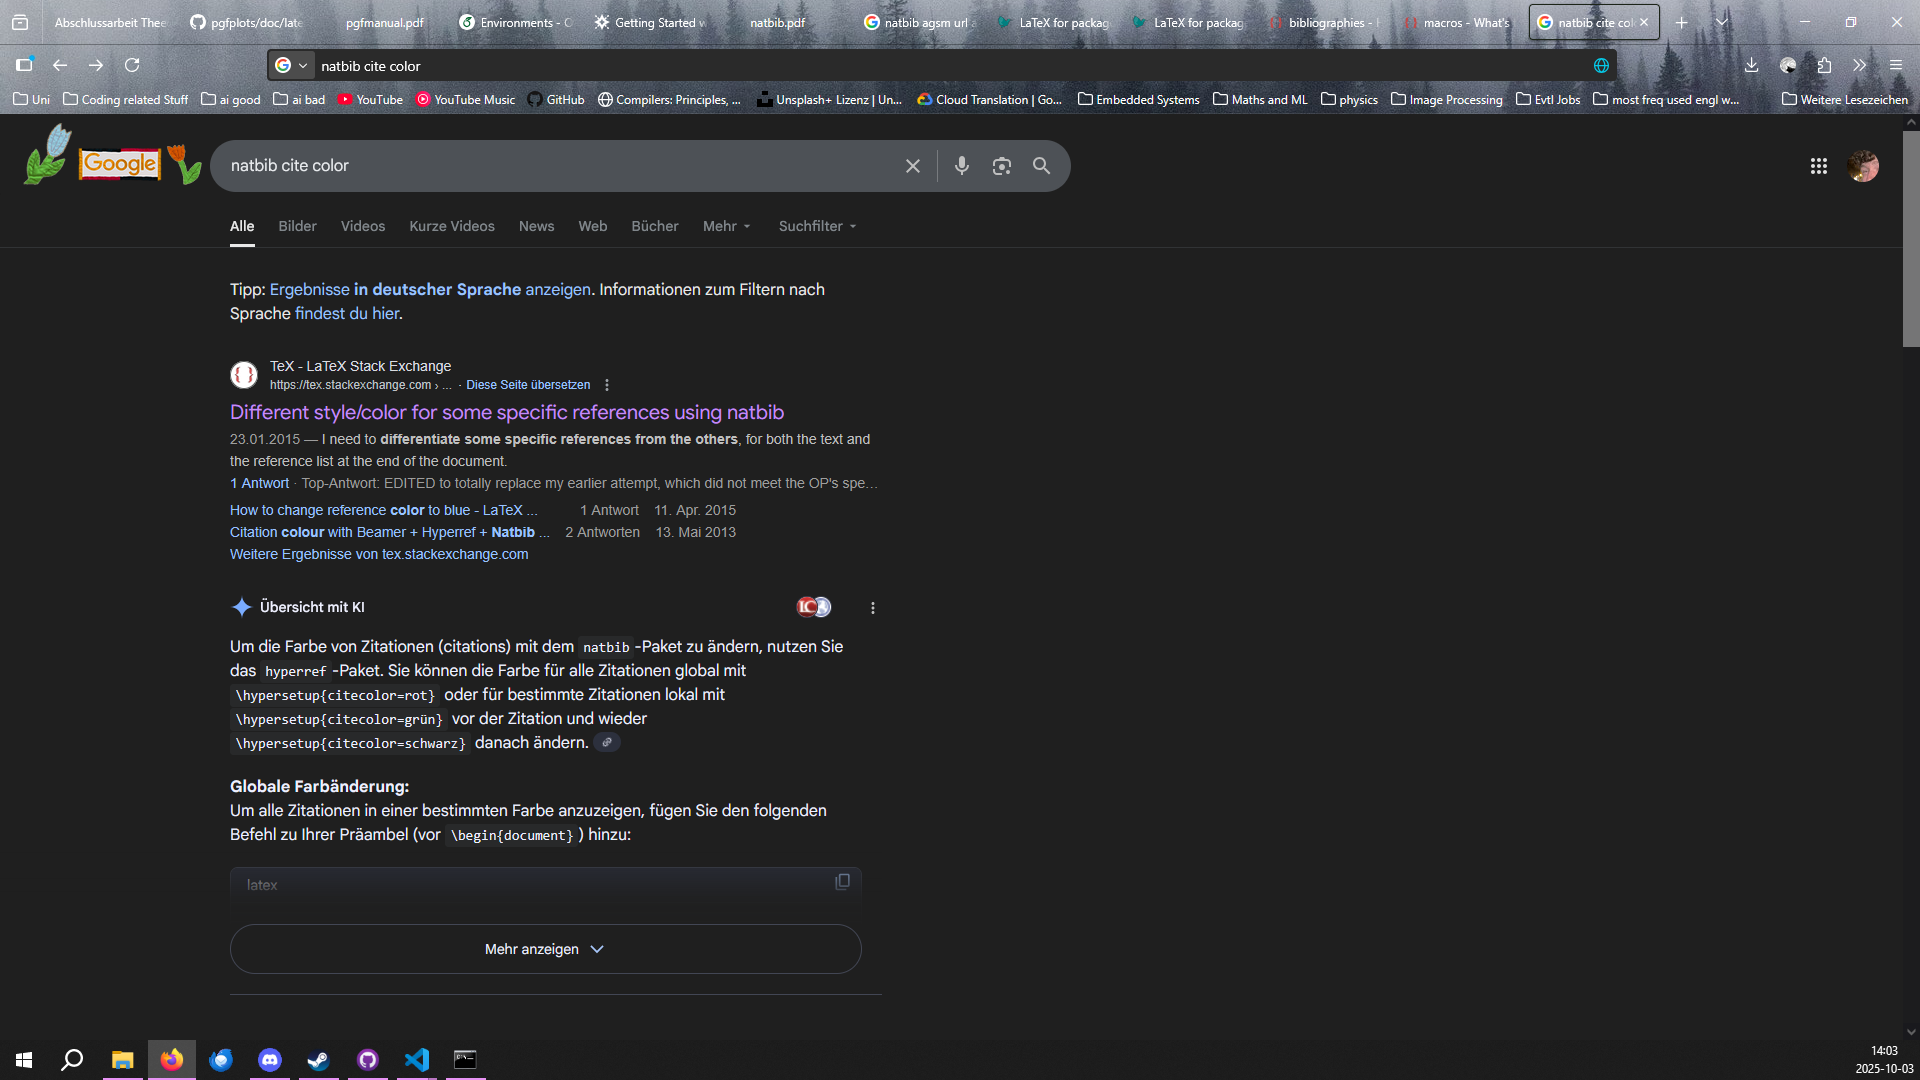
\includegraphics[width=\textwidth]{pictures/motivation.PNG}\label{fig:googlemakesmistakes}
\end{figure}
\endgroup

\end{document}